\chapter{Gestión y planificación}

\section{Metodología de desarrollo}
Es bien sabido que en el ámbito del desarrollo software durante décadas se han dado problemas como el no cumplimiento ni de requisitos, ni de estimaciones de tiempo y recursos. Son el surgimiento de estos problemas a lo que evocó a la creación de metodologías de desarrollo con el objetivo de evitar o minimizar dichos problemas. Así que, una \textbf{metodología de desarrollo} se define como un de marco de trabajo utilizado con el fin de estructurar y controlar un proceso de desarrollo. \bigskip

A continuación se muestra una tabla con los dos grupos en los que puede ser una metodología de desarrollo clasificada junto con sus respectivas diferencias:

\begin{table}[H]
\begin{tabular}{|l|l|}
\hline
\rowcolor[HTML]{EFEFEF} 
\multicolumn{1}{|c|}{\cellcolor[HTML]{EFEFEF}Metodologías tradicionales}                                                                              & \multicolumn{1}{c|}{\cellcolor[HTML]{EFEFEF}Metodologías ágiles}                                               \\ \hline
\begin{tabular}[c]{@{}l@{}}La fase de test de la aplicación \\ es realizada sólo una vez tras \\ ser la fase de desarrollo \\ completada\end{tabular} & \begin{tabular}[c]{@{}l@{}}La fase de test de la aplicación\\ es un proceso realizado de forma iterativa\end{tabular} \\ \hline
Sigue una organización lineal                                                                                                                         & Sigue una organización iterativa                                                                               \\ \hline
\begin{tabular}[c]{@{}l@{}}La participación del cliente\\ es menor\end{tabular}                                                                       & La participación del cliente es mayor                                                                          \\ \hline
\begin{tabular}[c]{@{}l@{}}Apoya un modelo de desarrollo\\ fijo\end{tabular}                                                                          & \begin{tabular}[c]{@{}l@{}}Apoya un modelo de desarrollo adaptable\\ al cambio\end{tabular}                    \\ \hline
Difícil la adaptación al cambio                                                                                                                       & Fácil adaptación al cambio                                                                                     \\ \hline
Gestión de equipo grandes                                                                                                                             & Gestión de equipos pequeños                                                                                    \\ \hline
\end{tabular}
\caption{Tabla de diferencias entre metodologías de desarrollo tradicional y ágil}
\end{table}

\subsection{SCRUM}
Para el desarrollo de este proyecto se ha elegido la metodología de desarrollo ágil SCRUM, pues es de las metodologías de desarrollo más utilizadas en la actualidad, de hecho empresas de gran calibre como Movistar, Google, Vodafone, Electronic Arts... utilizan dicha metodología. \bigskip

¿Qué es SCRUM? Es un marco de trabajo para el desarrollo de proyecto caracterizado por ser iterativo e incremental, así como adaptativo pues no sigue un plan lineal, sino una adaptación continua. Sus principios son la \textbf{transparencia}, la \textbf{inspección} y la \textbf{adaptación} cumpliendo con los valores de mejora continua, compromiso, calidad, simplicidad, respeto, coraje, ritmo y responsabilidad. \bigskip

Sabiendo previamente que un \textbf{Sprint} es un intervalo de tiempo comprendido entre 1 a 4 semanas, durante el que se crea un incremento del producto del proyecto ''terminado'' y utilizable, SCRUM se compone de los siguientes elementos:

\begin{itemize}
    \item \textbf{Artefactos}:
    \begin{itemize}
        \item \textbf{Pila del producto (Product Backlog)}: Es una lista de requisitos que ha sido priorizada de todas las funcionalidades y características que ha de cumplir el producto. 
        \item \textbf{Pila del Sprint (Sprint Backlog)}: Es la selección de requisitos del la Pila del Producto, se compone de tareas de desarrollo que expresan los requisitos en lenguaje técnico.
    \end{itemize}
    \item \textbf{Reuniones}:
    \begin{itemize}
        \item \textbf{Planificación del Sprint}: Es una reunión previa antes del comienzo del Sprint en la que se determina el objetivo del éste y las tareas a desarrollar.
        \item \textbf{Reunión diaria}: Se trata de una reunión realizada diariamente en la que cada miembro del equipo expone las tareas realizadas, así como los obstáculos encontrados.
        \item \textbf{Revisión del Sprint}: Es una reunión que tiene lugar el último día del Sprint cuyo objetivo es el de obtener información sobre el estado del proyecto.
        \item \textbf{Retrospectiva del Sprint}: Al final de cada Sprint se realiza una reunión de retrospectiva en la que se identifican los puntos fuertes a mantener y débiles a mejorar del equipo durante el desarrollo.
    \end{itemize}
    \item \textbf{Roles}:
        \begin{itemize}
        \item \textbf{Propietario}: Es el representante del cliente, debe de conocer los requisitos del cliente y tener cierta experiencia con los métodos utilizados por el equipo. Se encarga de recolectar los requisitos del cliente, resolver dudas del Equipo de Desarrollo y de priorizar la Pila del Producto, así como de aceptar o rechazar el software realizado al final una iteración.
        \item \textbf{Director del proyecto}: Promueve los valores de Scrum, se asegura de que el equipo es totalmente funcional y es su escudo del resto del equipo ante amenazas externas. Se encarga de asegurar que el Propietario conozca cómo ordenar la Pila del Producto para maximizar el valor, de guiar y ayudar al Equipo de Desarrollo y motivar a que se realicen cambios que incrementen la productividad.
        \item \textbf{Equipo de desarrollo}: Se forma por un conjunto de profesionales que se ocupan de entregar un incremento del producto del proyecto ''terminado'' al final de cada Sprint. Normalmente un Equipo de Desarrollo se forma entre 5-9 personas.
    \end{itemize}
\end{itemize}

\begin{figure}[H]
    \centering{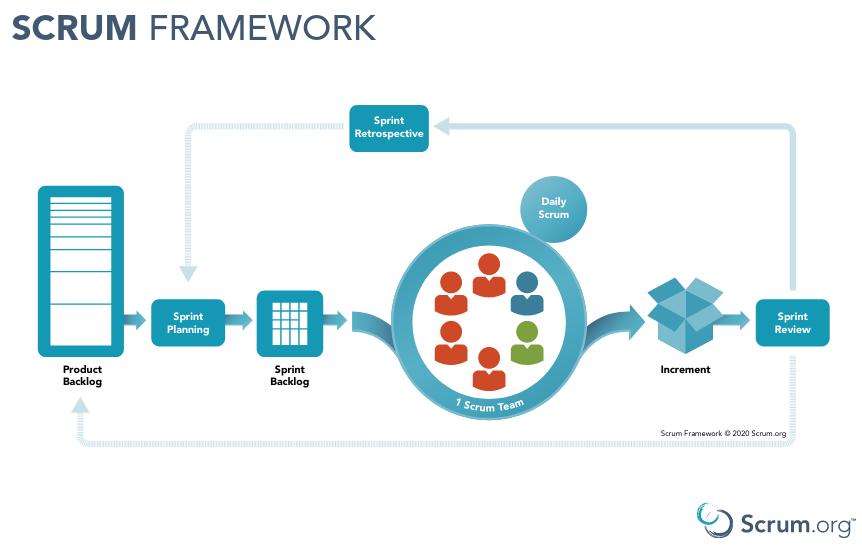
\includegraphics[scale=0.3]{doc/imagenes/scrum-esquema.png}}
    \caption{Esquema del marco de trabajo de SCRUM}
    \label{fig:scrum-esquema}
\end{figure}

\subsection{Aplicación de SCRUM a este proyecto}
Debido a que el desarrollo del proyecto se hará de forma individual, se debe de hacer una adaptación de SCRUM a la metodología de trabajo que se va a llevar a lo largo del proyecto.

\begin{itemize}
    \item Debido a que el Equipo de Desarrollo está compuesto por una sóla persona, las reuniones diaras son eliminadas.
    \item Al final de cada Sprint se tratará de acordar una reunión con la tutora en la que se hará una retrospectiva de éste y se establecerán nuevos objetivos.
\end{itemize}

\section{Gestión de la configuración}
En esta sección se indicará cómo se procederá para la gestión de la configuración de todos los elementos pertenecientes a este proyecto. Debido a que los elementos de trabajo que conforman el proyecto son el código y la documentación, a continuación se explicará la gestión de cada uno por separado.

\subsection{Gestión del código}
Para la gestión del código se procederá para asegurar su seguridad ante cualquier posible pérdida, la realización de backups PC y el uso de Git para el control de versiones en local y Github en la nube. Ambas herramientas son explicadas posteriormente en la sección \ref{recursos-software}. \bigskip

El código se dividirá en dos partes: frontend y backend. Por un lado, el backend será implementado en el lenguaje de programación Javascript haciendo uso de NodeJS para construir la API. Por otro lado, el frontend será implementado en el lenguaje Typescript haciendo uso de Angular y se utilizarán HTML, SCSS y Angular Material para construir la interfaz. Para cada parte se creará un repositorio en Github que se mantendrá en privado hasta el día de la presentación del proyecto.

\subsection{Gestión de la documentación}
Para la gestión de la documentación se creará un tercer repositorio en Github que se mantendrá en privado de igual forma hasta el día de la presentación del proyecto. En cuanto a la redacción de la documentación, ésta se realizará en la nube en el editor de LaTeX de Overleaf. Sin embargo, la herramienta requiere de un plan de pago para llevar a cabo la sincronización con Github, es por esto que se ha creado un repositorio en local con objeto de almacenar en el respositorio en remoto de Github éste.

\section{Gestión del tiempo}
Para alcanzar con los objetivos propuestos del proyecto se han definido una serie de épicas y tareas asociadas a ellas:
\begin{itemize}
    \item \textbf{E.1} Estado del arte de la gestión de citas online:
    \begin{itemize}
        \item \textbf{T.1.1}: Entrevista con la clínica Carmen Verdejo para conocer su gestión actual de citas.
        \item \textbf{T.1.2}: Investigación sobre las herramientas utilizadas en la clínica Carmen Verdejo.
        \item \textbf{T.1.3}: Buscar y leer literatura sobre gestión de citas online.
        \item \textbf{T.1.4}: Investigación de soluciones genéricas dedicadas a planificación.
        \item \textbf{T.1.5}: Investigación de soluciones específicas para la gestión de citas en centros sanitarios.
    \end{itemize}
    
    \item \textbf{E.2}: Implementación de un login para personal y pacientes:
    \begin{itemize}
        \item \textbf{T.2.1}: Investigación sobre cómo implementar un sistema de login.
        \item \textbf{T.2.2}: Definir y crear el modelo de la base de datos de los usuarios.
        \item \textbf{T.2.3}: Definir un sistema jerárquico de roles.
        \item \textbf{T.2.4}: Implementar en Backend un sistema de login.
        \item \textbf{T.2.5}: Diseñar la interfaz del login.
        \item \textbf{T.2.6}: Implementar el diseño realizado en T.2.3 en Frontend e implementar las llamadas al Backend.
    \end{itemize}
    
    \item \textbf{E.3}: Implementación de la vista principal:
    \begin{itemize}
        \item \textbf{T.3.1}: Investigar Angular Scheduler.
        \item \textbf{T.3.2}: Definir y crear el modelo de la base de datos de las citas.
        \item \textbf{T.3.3}: Diseñar la interfaz de la vista principal.
        \item \textbf{T.3.4}: Implementar de los endpoints para operaciones CRUD sobre citas en Backend utilizando el modelo de datos de Angular Scheduler.
        \item \textbf{T.3.5}: Implementar el diseño de T.3.3 e implementar las llamadas al Backend.
    \end{itemize}
    
    \item \textbf{E.4}: Implementación de las vistas del listado de personal y pacientes:
    \begin{itemize}
        \item \textbf{T.4.1}: Implementación de endpoints CRUD para los usuarios de la plataforma.
        \item \textbf{T.4.2}: Diseñar la vista del listado del personal.
        \item \textbf{T.4.3}: Diseñar la vista del listado de pacientes.
        \item \textbf{T.4.4}: Implementar las vistas de los diseños de T.4.2 y T.4.3.
    \end{itemize}
    
    \item \textbf{E.5}: Implementación de la vista de ajustes:
    \begin{itemize}
        \item \textbf{T.5.1}: Diseñar la vista de ajustes.
        \item \textbf{T.5.2}: Añadir los endpoints de ajustes al Backend.
        \item \textbf{T.5.3}: Implementar en Frontend el diseño de T.5.1.
    \end{itemize}

    \item \textbf{E.6}: Implementación de pruebas de unidad e integración:
    \begin{itemize}
        \item \textbf{T.6.1}: Definición de las pruebas de unidad e integración.
        \item \textbf{T.6.2}: Implementación de las pruebas de unidad.
        \item \textbf{T.6.3}: Implementación de las pruebas de integración.
    \end{itemize}   
\end{itemize}

\subsection{Planificación temporal}
\begin{figure}[H]
    \centering{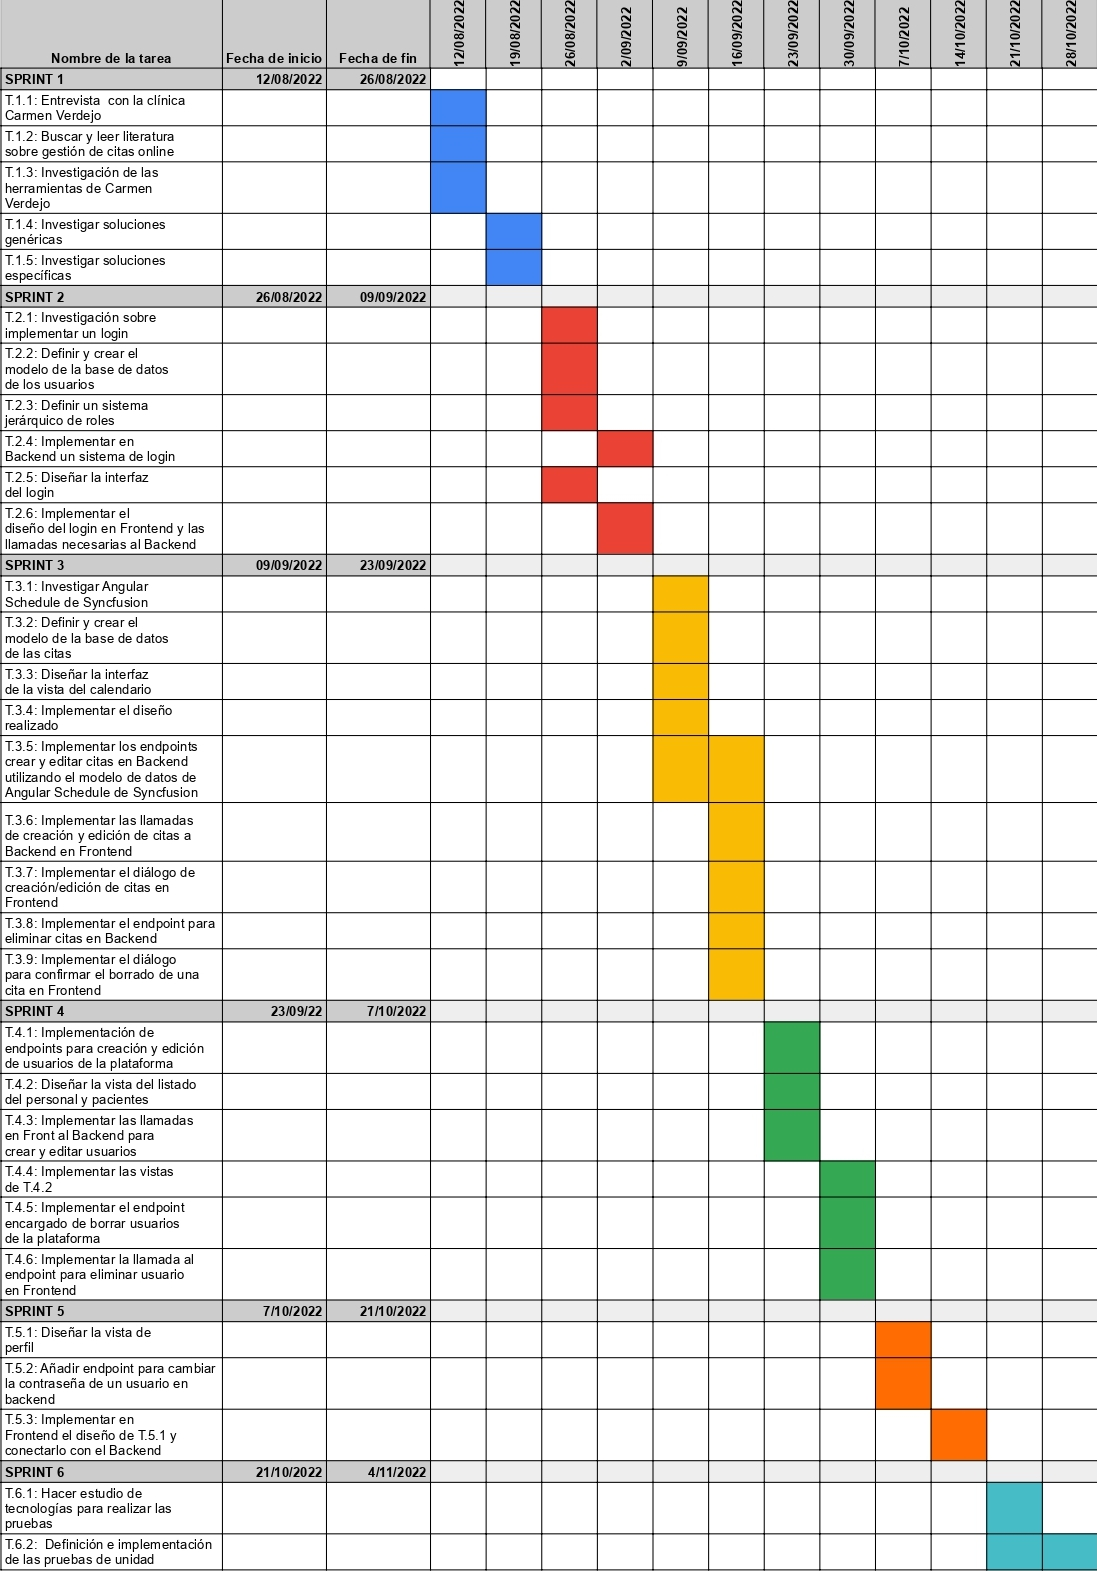
\includegraphics[scale=0.5]{doc/imagenes/gantt.jpg
    }}
    \caption{Diagrama de Gantt de la planificación temporal}
    \label{fig:gantt}
\end{figure}

Además de estas tareas, durante el desarrollo del proyecto se redactará toda la documentación correspondiente a éste.

\section{Gestión de recursos} \label{recursos}
\subsection{Recursos humanos}
\begin{itemize}
    \item \textbf{Dña. Rocío Celeste Romero Zaliz}, profesora del Departamento de Ciencias de la Computación e Inteligencia Artificial de la Universidad de Granada como tutora del proyecto.
    \item \textbf{Inés Nieto Sánchez}, estudiante del grado en Ingeniería Informática en la Escuela Técnica Superior de Ingenierías Informática y Telecomunicación.
\end{itemize}

\subsection{Recursos materiales}
Los recursos utilizados para este Trabajo de Fin de Grado han sido muy pocos, en concreto sólo se ha utilizado el portátil personal:
\begin{itemize}
    \item \textbf{MSI Modern 14 A10M}: Se trata de un portatil de la marca MSI con un procesador Comet Lake i7-10510U con una memoria RAM de 16GB y una arquitectura de 64 bits. Todo el desarrollo del proyecto, así como la documentación correspondientes serán realizados haciendo uso de este portátil.
\end{itemize}
\subsection{Recursos software} \label{recursos-software}
En cuanto a los recursos software se ha optar por la utilización de software de código abierto y recurrir a las licencias gratuitas ofrecidas al estudiantado para disminuir lo máximo posible el coste del proyecto. A continuación se expone el listado de los recursos software utilizados:

\begin{itemize}
    \item \textbf{Elementary OS}: Se trata de una distribución de código abierto del sistema operativo Linux.
    \item \textbf{WebStorm}: Es una IDE dedicada sobretodo al desarrollo web en JavaScript y Typesrcipt. Pertenece a la empresa de desarrollo software JetBrains y a pesar de que todas las IDEs desarrolladas por JetBrains son de pago, se hará uso de la licencia gratuita ofrecida a estudiantes.
    \item \textbf{Git}: Se trata de un software de control de versiones.
    \item \textbf{Github}: Es una plataforma cuyo servicio es el de alojar el sistema de control de versión Git.
    \item \textbf{Docker}: Es una herramienta de código abierto diseñada con objeto de automatizar el despliegue de aplicaciones en contenedores software.
    \item \textbf{NodeJS}:Es un entorno de código abierto utilizado para hacer uso de JavaScript ejecutar JavaScript fuera del navegador.
    \item \textbf{Angular}: Es un framework de código abierto desarrollado por Google utilizado para creer aplicaciones web y móviles.
\end{itemize}

\subsection{Recursos  de comunicación y documentación}
Para la correcta evolución del proyecto se han de hacer uso de recursos para la comunicación entre sus participantes, así como el uso de herramientas utilizadas para la documentación del mismo.

\begin{itemize}
    \item \textbf{Overleaf}: Es un editor gratuito de LaTeX en la nube, utilizado para la documentación del proyecto.
    \item \textbf{Jira}: Software dedicado a la gestión de proyectos, se utilizará su plan grautito para la gestión del proyecto siguiendo una metodología SCRUM.
    \item \textbf{Visual Paradigm}: Es una aplicación software cuyo objetivo es el de modelado de sistemas de información y procesos de gestión de desarrollo. Se trata de una herramienta de pago, pero la Universidad de Granada ofrece a su estudiantado licencias gratuitas.
    \item \textbf{Draw.io}: Es un software online gratuito desarrollado por Google utilizado para la creación de diagramas y esquemas.
    \item \textbf{Google slides}: Es una herramienta desarrollada por Google para la creación y edición de presentaciones. Será utilizada para la elaboración de la presentación del proyecto.
    \item \textbf{Google meet}: Es un servicio de videoconferencia desarrollado por Google.
    \item \textbf{Correo UGR}: Es un servicio de correo electrónico de la UGR.
\end{itemize}

\section{Gestión de costes}
En esta sección se elaborará un presupuesto de acuerdo a los recursos explicados en la sección \ref{recursos} junto con los costes adicionales que supone el desarrollo del proyecto.

\subsection{Costes de recursos humanos}
Para los costes de recursos humanos, hemos de tener en cuenta que el equipo de desarrollo está formado por una persona que tomará el rol de Ingeniera Informática. Para estimar el coste del trabajo de dicho rol a continuación se hará un desglose del número de horas totales a trabajar y su coste. \bigskip

El proyecto se encuentra planteado para ser realizado en un período de 3 meses, es decir, 12 semanas. 

\begin{center}
$Dias\ naturales\ =\ 3\ meses\ *\ 30\ dias / mes\ =\ 90\ dias$
\end{center}

A este número de días naturales habrá que descontarle fines de semana:

\begin{center}
$Dias\ no \ laborales\ =\ 3\ meses\ *\ 8\ dias / mes\ =\ 24\ dias$
\end{center}

Resultando ser los días laborales invertidos en el desarrollo del proyecto los siguientes:

\begin{center}
$Dias\ laborales\ =\ 90\ dias\ -\ 24\ dias =\ 66 \ dias$
\end{center}

En cuanto a las horas trabajadas, una jornada laboral completa se constituye de 40 horas semanales. Sin embargo, debido a que la estudiante trabaja en paralelo con una jornada parcial durante la realización del proyecto, las horas semanales dedicadas son reducidas a 30 horas distribuidas en 6 horas diarias. Por tanto, el total de horas trabajadas es el siguiente:

\begin{center}
$Horas\ laborales\ =\ 66\ dias\ *\ 6 \ horas\ día = \ 396 \ horas$
\end{center}

Después de haber obtenido las horas laborales totales, el salario como ingeniero informático se ha obtenido en base al salario anual indicado por la Universidad Alfonso X El Sabio \footnote{\url{https://www.uax.com/blog/ingenieria/cuanto-cobra-un-ingeniero-informatico}}. Según la universidad madrileña un de un ingeniero informático con menos de 3 años de experiencia gana aproximadamente 20.450 euros anuales, en otras palabras, 1.704 euros mensuales que son 9,68 euros/hora. Así pues los costes de recursos humanos totales son:

\begin{center}
$Costes\ de \ recursos \ humanos \ =\ 396\ horas\ *\ 9.68 \ euros\ hora = \ 3.833,28 \ euros$
\end{center}

\subsection{Costes de recursos materiales}
Una vez hemos calculado los costes de recursos humanos, es momento de calcular los costes de recursos materailes. Para su cálculo se deberá de tener en cuenta que los recursos sufren de un fenómeno llamado \textit{depreciación} el cual hace que estos sean devaluados con el paso del tiempo. 

Como se ha expuesto en la sección x PC sólo se utilizará una sóla herramienta, el portátil personal de la estudiente. Para calcular su actual precio se aplicará el método de depreciación lineal usado para conocer la reducción del valor de un bien. 

Para calcular la depreciación se deberá antes calcular el valor residual del dispositivo el cual es el valor que poseerá al final de la vida útil del mismo. Suponemos para ello, que la vida útil de un portátil es de 5 años: 

\begin{equation}
    Valor\ residual = \frac{Coste\ inicial}{Vida\ util\ (a\tilde{n}os)} = \frac{899 \ \EUR}{5 \ a\tilde{n}os} = 179,8\ \EUR{}
\end{equation}

 Una vez conocido el valor residual, la depreciación se calcula de la siguiente forma:
\begin{equation}
    Depreciacion = \frac{Coste \ inicial - Valor\ residual}{Vida\ util\ ( a\tilde{n}os)} = \frac{899\EUR \ - \ 179,8\EUR }{5 \ a\tilde{n}os} = 143,84\ \EUR{}
\end{equation}

\begin{table}[H]
\begin{tabular}{|l|l|l|l|c|}
\hline
\textbf{Recurso}                        & \textbf{Valor inicial (€)} & \textbf{Valor residual (€)} & \textbf{Antigüedad (años)} & \multicolumn{1}{l|}{\textbf{Valor actual (€)}} \\ \hline
\multicolumn{1}{|c|}{Portátil personal} & \multicolumn{1}{c|}{899}   & \multicolumn{1}{c|}{179.8}  & \multicolumn{1}{c|}{4}     & 323,64                                         \\ \hline
\textbf{TOTAL}                          &                            &                             &                            & 323,64                                         \\ \hline
\end{tabular}
\caption{Tabla de los costes materiales}
\end{table}

\subsection{Costes de recursos software, comunicación y documentación}
Los costes referentes a los recursos software son nulos puesto que todos son de código abierto, a excepción de WebStorm que no es gratutito, sin embargo su propietario JetBrains dispone de licencias gratuitas para estudiantes. Por otro lado, en lo que respecta a los recursos utilizados para la documentación y comunicación son totalmente gratuitos salvo Visual Paradigm el cual es utilizado por una licencia gratuita ofrecida por la UGR.


\subsection{Costes adicionales}
Dentro de los costes adicionales se encuentran aquellos costes que no se han nombrado en los apartados anteriores, pero han sido necesarios para el desarrollo del proyecto. Estos costes son correspondientes a la factura de la luz e Internet:


\begin{table}[H]
\centering
\begin{tabular}{cc}
\hline
\multicolumn{1}{l}{\textbf{Recurso}} & \multicolumn{1}{l}{\textbf{Importe (€/mes)}} \\ \hline
Luz                                  & 25                                           \\
Internet                             & 70                                           \\ \hline
\end{tabular}
\caption{Tabla de los costes adicionales}
\end{table}

\subsection{Presupuesto total}
En la siguiente tabla se presenta la visión global de los costes de este proyecto:

\begin{table}[H]
\centering
\begin{tabular}{lc}
\hline
\textbf{Recurso}                                                                                      & \multicolumn{1}{l}{\textbf{Importe}} \\ \hline
\textbf{Costes de recursos humanos}                                                                   & \multicolumn{1}{l}{}                 \\
Trabajo autónomo                                                                                      & 3.833,28€                            \\ \hline
\textbf{Costes de recursos materiales}                                                                & \multicolumn{1}{l}{}                 \\
Portátil personal                                                                                     & 323,64€                              \\ \hline
\textbf{Costes de recursos software}                                                                  & \multicolumn{1}{l}{}                 \\
Elementary OS                                                                                         & 0,0€                                 \\
WebStorm                                                                                              & 0,0€                                 \\
Git                                                                                                   & 0,0€                                 \\
Github                                                                                                & 0,0€                                 \\
Docker                                                                                                & 0,0€                                 \\
NodeJS                                                                                                & 0,0€                                 \\
Angular                                                                                               & 0,0€                                 \\ \hline
\textbf{\begin{tabular}[c]{@{}l@{}}Costes de recursos de\\ comunicación y documentación\end{tabular}} & \multicolumn{1}{l}{}                 \\
Draw.io                                                                                               & 0,0€                                 \\
Overleaf                                                                                              & 0,0€                                 \\
Visual Paradigm                                                                                       & 0,0€                                 \\
Google Meet                                                                                           & 0,0€                                 \\
Correo UGR                                                                                            & 0,0€                                 \\
Joplin                                                                                                & 0,0€                                 \\ \hline
\textbf{Costes adicionales}                                                                           & \multicolumn{1}{l}{}                 \\
Factura de la luz                                                                                     & 25€                                  \\
Factura de Internet                                                                                   & 70€                                  \\ \hline
\textbf{TOTAL}                                                                                        & \multicolumn{1}{l}{4.251,92€}       
\end{tabular}
\caption{Tabla del presupuesto total del proyecto}
\end{table}

\section{Gestión de riesgos}
Durante el desarrollo de todo proyecto se tiene siempre la posibilidad de que puedan manifestarse ciertas situaciones que supongan un obstáculo o incluso amenaza para su correcta evolución. Es por ello que por mínima que sea la posibilidad de que ocurran hay que estar preparado y para ello se debe de precisar un plan de actuación.

En esta sección se identificarán los posibles riesgos a correr durante el proyecto, sus causas y el plan de actuación en caso de ser materializados para solventar o reducir lo máximo posible su impacto. Posteriormente se hará una estimación de la probabilidad de aparición y del impacto que supone cada uno de ellos.

\subsection{Identificación de riesgos}
\begin{figure}[H]
    \centering{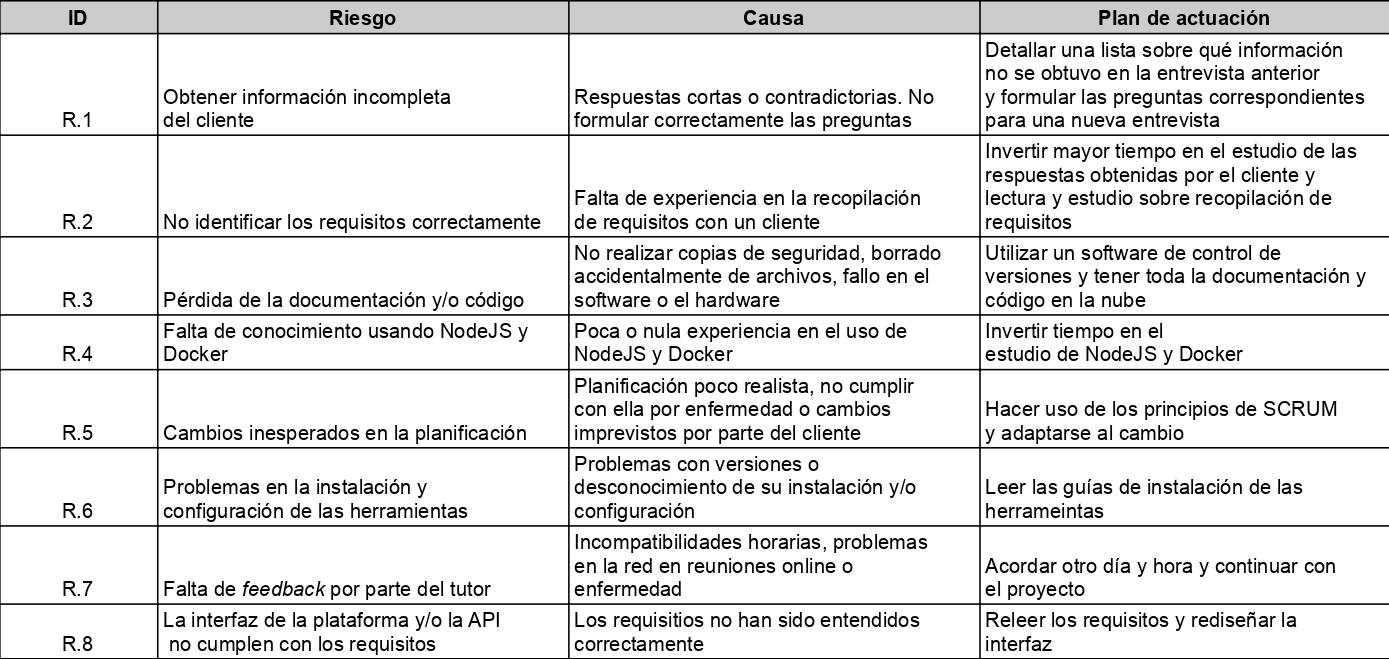
\includegraphics[scale=0.6]{doc/imagenes/riesgos.jpg}}
    \caption{Tabla de riesgos del proyecto}
    \label{fig:riesgos}
\end{figure}
\subsection{Análisis de riesgos}
Para analizar los riesgos expuestos anteriormente, se ha hecho uso de una matriz de probabilidad-impacto:

\begin{figure}[H]
    \centering{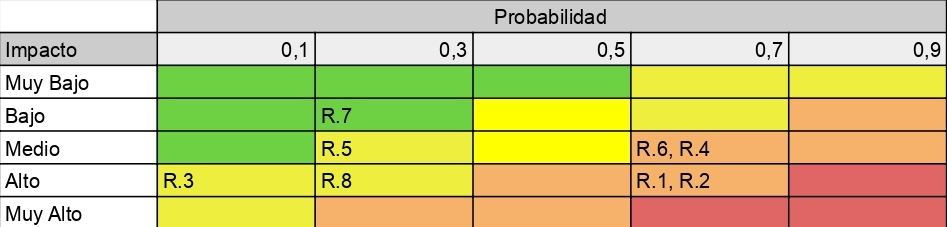
\includegraphics[scale=0.6]{doc/imagenes/analisis-riesgos.jpg}}
    \caption{Matriz de probabilidad-impacto de riesgos}
    \label{fig:analisis-riesgos}
\end{figure}

\subsection{Riesgos materializados}
Los riesgos surgidos durante el transcurro del desarrollo del proyecto han sido precisamanete los marcados con mayor probabilidad en la matriz de probabilidad-impacto \ref{fig:analisis-riesgos} (R.1, R.2, R.4 y R.6) . La falta de experiencia ante el reto que supone recoger información de un cliente ha provocado que surgieran numerosas dudas acerca de los requisitos del proyecto. A su vez la utilización de Docker y NodeJS por primera vez ha evocado a invertir gran parte del tiempo del primer sprint en su instalación y estudio. \bigskip

A pesar de la manifestación de los riesgos nombrados se ha sabido aplicar correctamente el plan de actuación previamente establecido para cada uno.